

%-------------------------------------------------------------------------------
% Dokumenten Klasse
\documentclass[
	final,
	a4paper,
	oneside,
	parskip=full,
	headings=standardclasses,
	headings=big,
	pointednumbers
]{scrartcl}

%-------------------------------------------------------------------------------
% Packete nutzen
\usepackage{ngerman,palatino,setspace}
\usepackage[T1]{fontenc}
\usepackage[latin9]{inputenc}
\usepackage[left=35mm,right=35mm,top=25mm,bottom=25mm]{geometry}
\usepackage{graphicx}
\usepackage{scrpage2}
\usepackage{listings}
\usepackage[usenames,dvipsnames,svgnames]{xcolor}
\usepackage[hidelinks]{hyperref}
\usepackage{amsmath}
\usepackage{caption}

%-------------------------------------------------------------------------------
% Kopf- und Fusszeile

\pagestyle{scrheadings}
\clearscrheadfoot
\chead{Projekt 2: Nichtlineare System Identifikation}
\cfoot[Seite \thepage]{Seite \thepage}

%-------------------------------------------------------------------------------
%
\title{Projekt 2: Nichtlineare System Identifikation}
\subtitle{MND2}
\author{Andreas Bachmann \\ \href{mailto:bachman0@students.zhaw.ch}{bachman0@students.zhaw.ch}}
\date{\today}

%-------------------------------------------------------------------------------
% Dokumenten Einstellungen

% Section Abst�nde
\RedeclareSectionCommand[
	beforeskip=-1\baselineskip,
	afterskip=0.001\baselineskip
]{section}
\RedeclareSectionCommand[
	beforeskip=0\baselineskip,
	afterskip=0.001\baselineskip
]{subsection}

% Formeln
\DeclareCaptionType{mycapequ}[aa][bb]
\captionsetup[mycapequ]{labelformat=empty}

%-------------------------------------------------------------------------------
% Listings
\lstset{
	language=Matlab,
	breaklines=true,
	numbers=left,
	numberstyle=\tiny,
	numbersep=5pt,
	captionpos=b,
	basicstyle=\footnotesize\ttfamily,
	stringstyle=\color{magenta},
	identifierstyle=\color{black},
	keywordstyle=\color{blue}, 
	commentstyle=\color{DarkGreen}
}

\newcommand{\mylisting}[2][]{%
	\lstinputlisting[caption={\texttt{\detokenize{#2}}},#1]{#2}%
}

%-------------------------------------------------------------------------------
% Dokument
\begin{document}
	\maketitle
	
	\section*{Aufgabe 1}
	Berechnen Sie mit Hilfe der Methode nach Runge numerisch eine L�sung der DGL.
	\begin{mycapequ}[!ht]
		\begin{align*}
		d = 1,\; l = 1,\; k = \frac{g}{l} = \frac{9.81}{1} \\
		\alpha = \varphi_{0},\; t \in \left[ 0, \; 4 \right] 
		\end{align*}
	\end{mycapequ}

	wobei  $ \phi_{0} = 3.14 $ der erste Messwert der Daten ohne Rauschen sei. Stellen Sie die L�sung
	jeweilen in einem eigenen Phasendiagramm dar.
	
	\subsection*{L�sung}
	
	\begin{mycapequ}[!ht]
		\begin{align*}
		    \varphi            & = \varphi_{0}  = phi \left(1\right) \\
			\dot{\varphi}      & = \varphi_{1}  = \dot{\varphi_{0}} = phi \left(2\right) \\
			\\
			\varphi_{d}        & = \varphi_{2}  = phi \left(3\right) \\
			\dot{\varphi_{d}}  & = \varphi_{3}  = \dot{\varphi_{2}} = phi \left(4\right) \\
			\\
			\varphi_{k}        & = \varphi_{4}  = phi \left(5\right) \\
			\dot{\varphi_{k}}  & = \varphi_{5}  = \dot{\varphi_{4}} = phi \left(6\right) \\
		\end{align*}
		\vspace{-0.75cm}
	\end{mycapequ}
	
	
	
	\begin{figure}[htbp] 
		\centering
		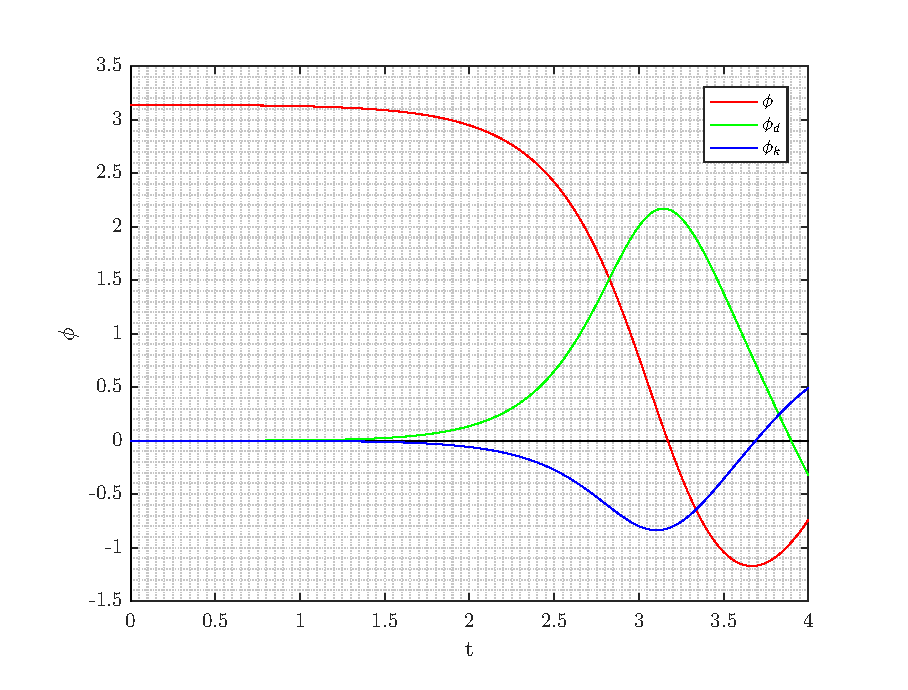
\includegraphics[width=0.7\textwidth]{aufgabe1_t.eps}
		\vspace{-10pt}
		\caption{Zeitdiagramm}
		\label{fig:t1}
	\end{figure}
	\begin{figure}[htbp] 
		\centering
		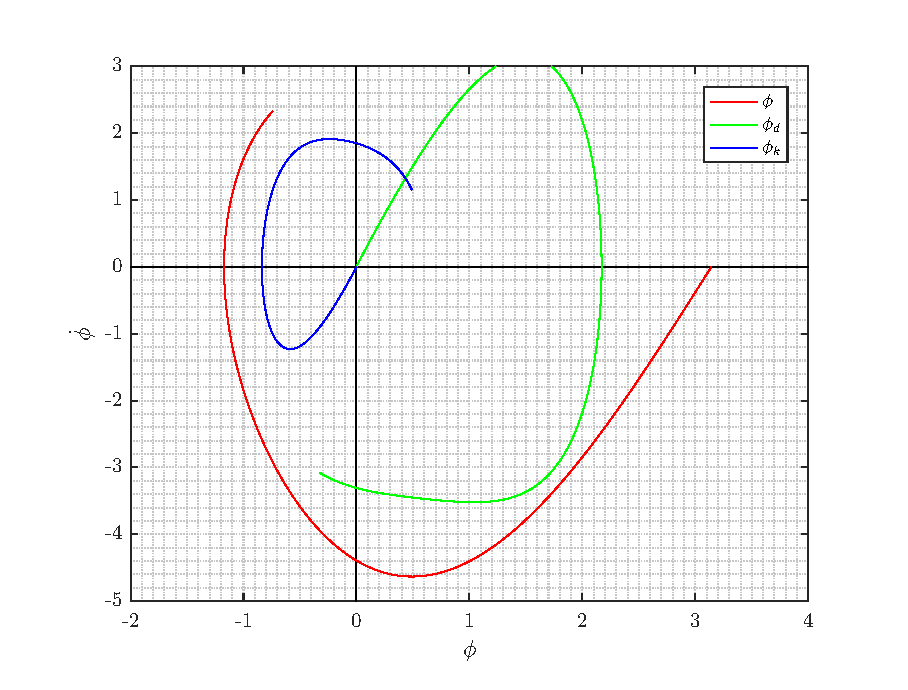
\includegraphics[width=0.7\textwidth]{aufgabe1_phase.eps}
		\vspace{-10pt}
		\caption{Phasenkurve}
		\label{fig:phase1}
	\end{figure}
	
	\newpage
	
	\section*{Aufgabe 3}
	Implementieren Sie das Levenberg-Marquardt Verfahren f�r das nichtlineare Ausgleichsproblem
	Welche Werte f�r die Parameter $ d, \, k $ sind d�r die ideale Messung optimal?
	
	\subsection*{L�sung}
	
	
	\begin{mycapequ}[!ht]
		\begin{align*}
		d_{Harmonic}       & = 1.7835 \\
		k_{Harmonic}       & = 68.4893 \\
		\\
		d_{Noisy}          & = 1.9172 \\
		k_{Noisy}          & = 69.1499
		\end{align*}
	\end{mycapequ}

	\begin{figure}[htbp] 
		\centering
		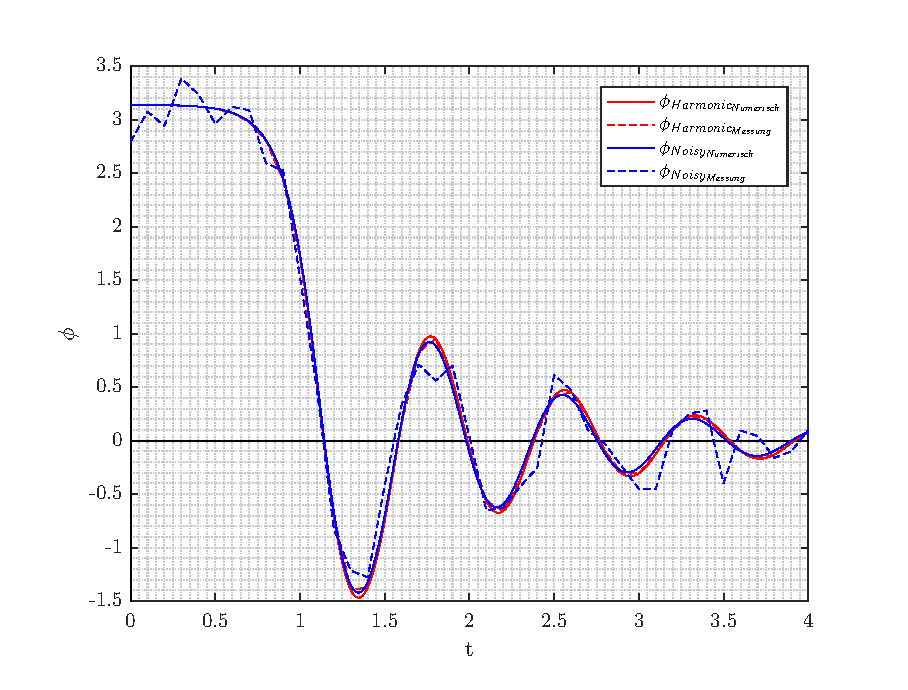
\includegraphics[width=0.7\textwidth]{aufgabe3_t.eps}
		\vspace{-10pt}
		\caption{Zeitdiagramm}
		\label{fig:t2}
	\end{figure}
	\begin{figure}[htbp] 
		\centering
		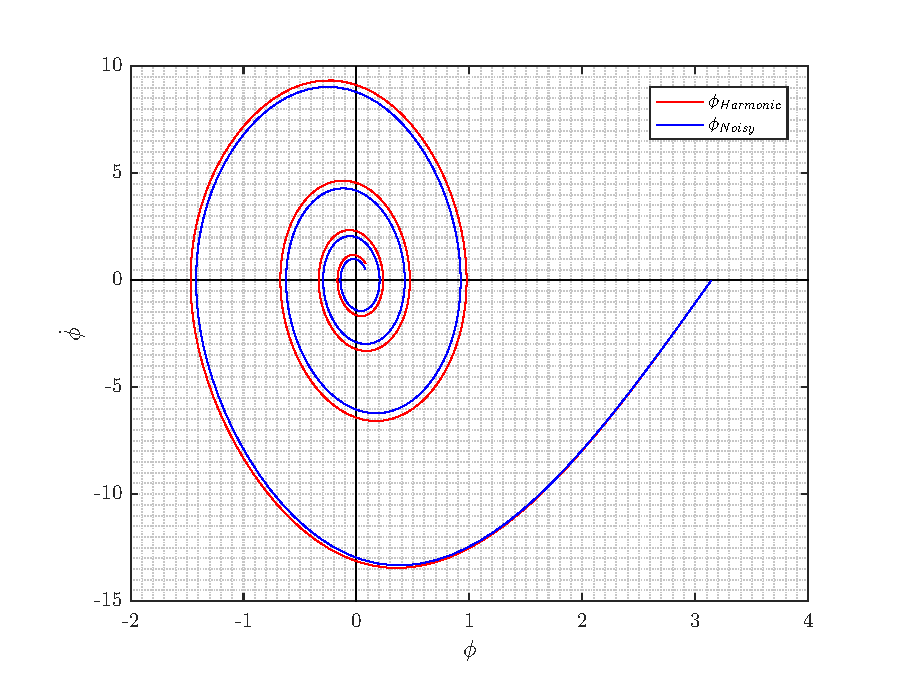
\includegraphics[width=0.7\textwidth]{aufgabe3_phase.eps}
		\vspace{-10pt}
		\caption{Phasenkurve $\varphi$}
		\label{fig:phase2}
	\end{figure}
	\begin{figure}[htbp] 
		\centering
		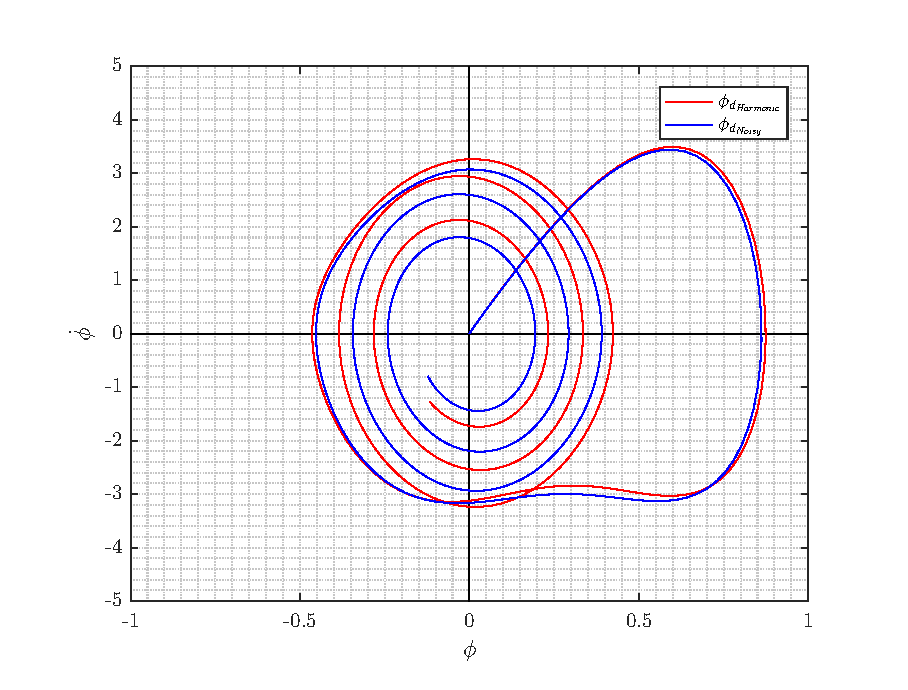
\includegraphics[width=0.7\textwidth]{aufgabe3_d_phase.eps}
		\vspace{-10pt}
		\caption{Phasenkurve $\varphi_{d}$}
		\label{fig:phase3}
	\end{figure}
	\begin{figure}[htbp] 
		\centering
		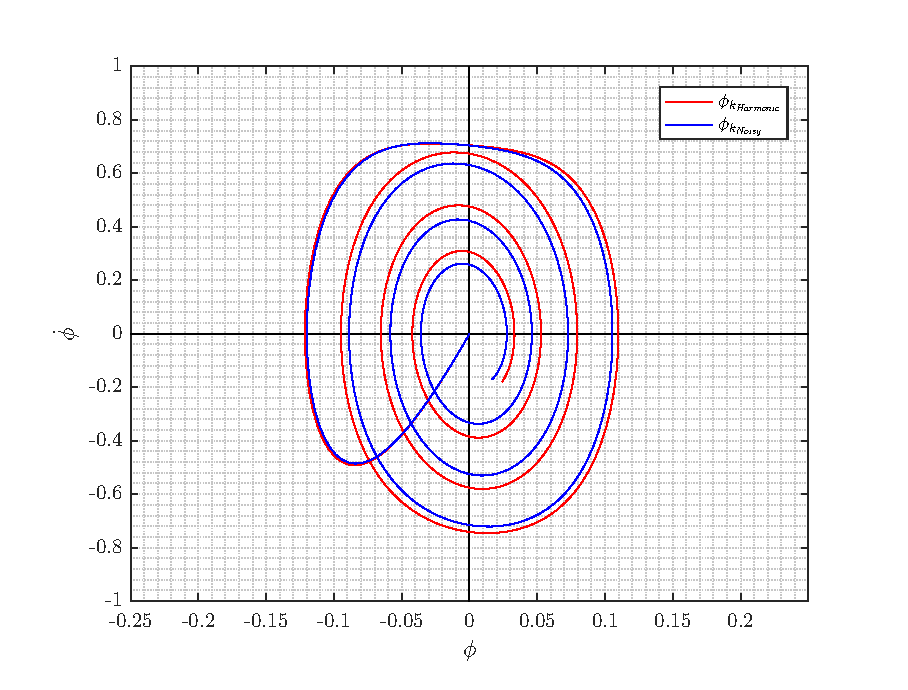
\includegraphics[width=0.7\textwidth]{aufgabe3_k_phase.eps}
		\vspace{-10pt}
		\caption{Phasenkurve $\varphi_{k}$}
		\label{fig:phase3}
	\end{figure}
	
		
\end{document}